\begin{figure}[t]
    \centering
    \begin{subfigure}[b]{0.49\textwidth}
        \centering
        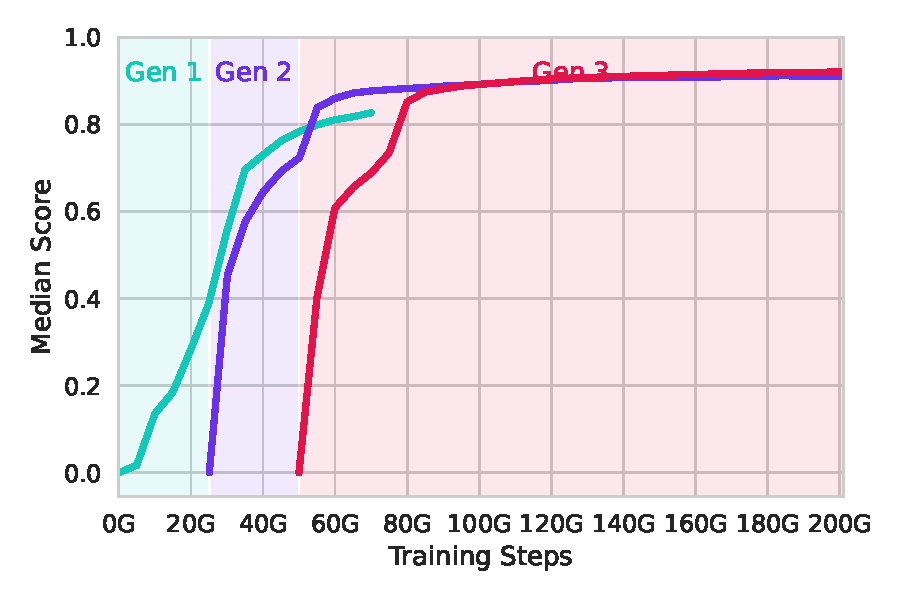
\includegraphics[width=\linewidth]{figures/distillation/distilation_3gen_percentile50_False.pdf} 
        \vskip -3pt \caption{}
    \end{subfigure}
    \begin{subfigure}[b]{0.49\textwidth}
        \centering
        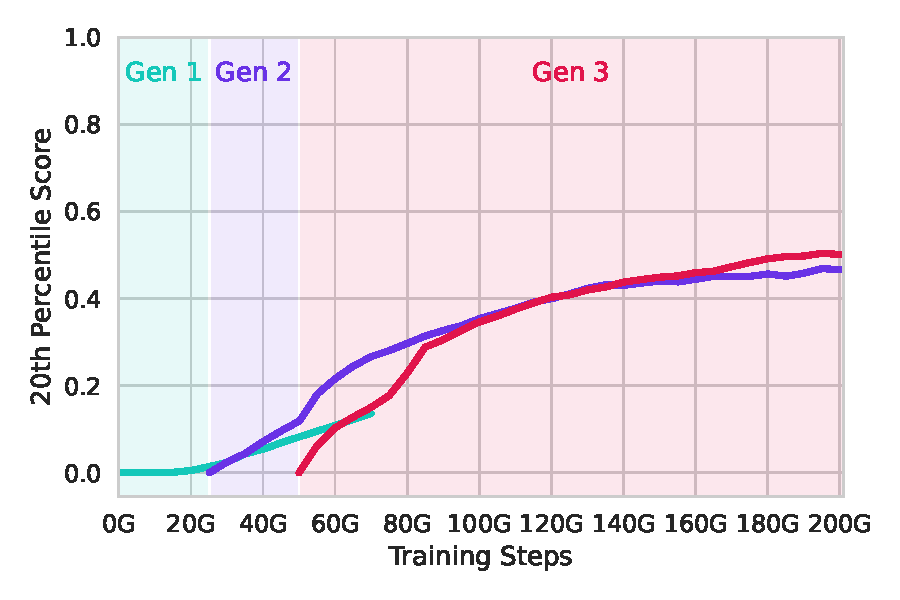
\includegraphics[width=\linewidth]{figures/distillation/distilation_3gen_percentile20_False.pdf}  
        \vskip -3pt \caption{}
    \end{subfigure}
    \caption{
        Normalised few-shot score over three generations using the 23M parameter Transformer-XL. The first and second generations correspond to the agents shown in Figure~\ref{fig:distillation}. The third generation is distilled from the second after it has been trained for 25 billion steps. The $x$-axis counts the combined amount of experience, starting from the experience collected by the original teacher. The third generation shows additional gains over the second, but to a lesser degree than the gap between the first and second generations.
    }
    \label{fig:app_distillation}
\end{figure}
\subsection{Repeated distillation}
\label{app:repeated_distillation}
In Section~\ref{sec:results_kickstarting}, we show that distilling an agent into an identical student can lead to large increases in the agent's performance. Here, we investigate the potential benefits of applying the procedure repeatedly. To this end, we continue the experiment shown in Figure~\ref{fig:distillation} and add a third generation, using a snapshot taken from the previous student after 25 billion frames, equivalent to 50 billion frames of total experience when taking the teacher's experience into account. Figure~\ref{fig:app_distillation} shows that applying this procedure repeatedly can indeed lead to additional benefits; however, we observe diminishing returns with successive generations. 